\section{Introduction}
\label{sec:introduction}

\ac{fl} is an advanced distributed machine learning paradigm that trains a model based on locally-trained gradients on the users side, then the gradients are collected from the users by a server for aggregation in an attempt to create a generic public model.
However, there is a privacy risk of learning important information about the data used by the users to train the model from their shared gradients.
\ac{ppfl} addresses these risks using cryptographic primitives for secure aggregation.
However, \ac{ppfl} faces challenges, notably vulnerability to model poisoning attacks that manipulate local updates to degrade model performance
Model poisoning attacks, led by Byzantine adversaries, can mislead the learning outcome and significantly impact \ac{fl} accuracy.


The challenges in designing an effective defense strategy against model poisoning attacks in \ac{ppfl} are multifaceted.
Firstly, encrypted model poisoning presents a covert threat as it conceals malicious gradients using encrypted gradients, making detection difficult.
Current defense strategies struggle to prevent encrypted model poisoning, especially when identifying malicious gradients without learning statistical distributions in \ac{ppfl}.
This allows encrypted poisonous gradients to evade existing defenses.
Secondly, there is a risk of privacy leakage in \ac{ppfl}, as some defense strategies may compromise privacy by accessing local gradients during model poisoning attack defense.
Thirdly, the unpredictability introduced by heterogeneous data, including \ac{iid} and non-\ac{iid} data, poses challenges.
While benign gradients from local \ac{iid} data exhibit a similar distribution, making anomalies detectable, gradients from non-\ac{iid} data are divergent, making it challenging for existing defense strategies to identify poisonous gradients.

\subsection{Related Work}
\label{sec:related-work}

\Cref{fig:comparison-with-state-of-the-art-schemes} presents a comparison between the proposed scheme and state-of-the-art schemes.
It shows that ShieldFL in the only scheme that works in both \ac{iid} and non-\ac{iid} settings while ensuring the full privacy of the gradients submitted by the users.
It can also solve malicious users byzantine behavior, where they can launch any kind of attacks. 

\begin{figure}[thb]
\centering
  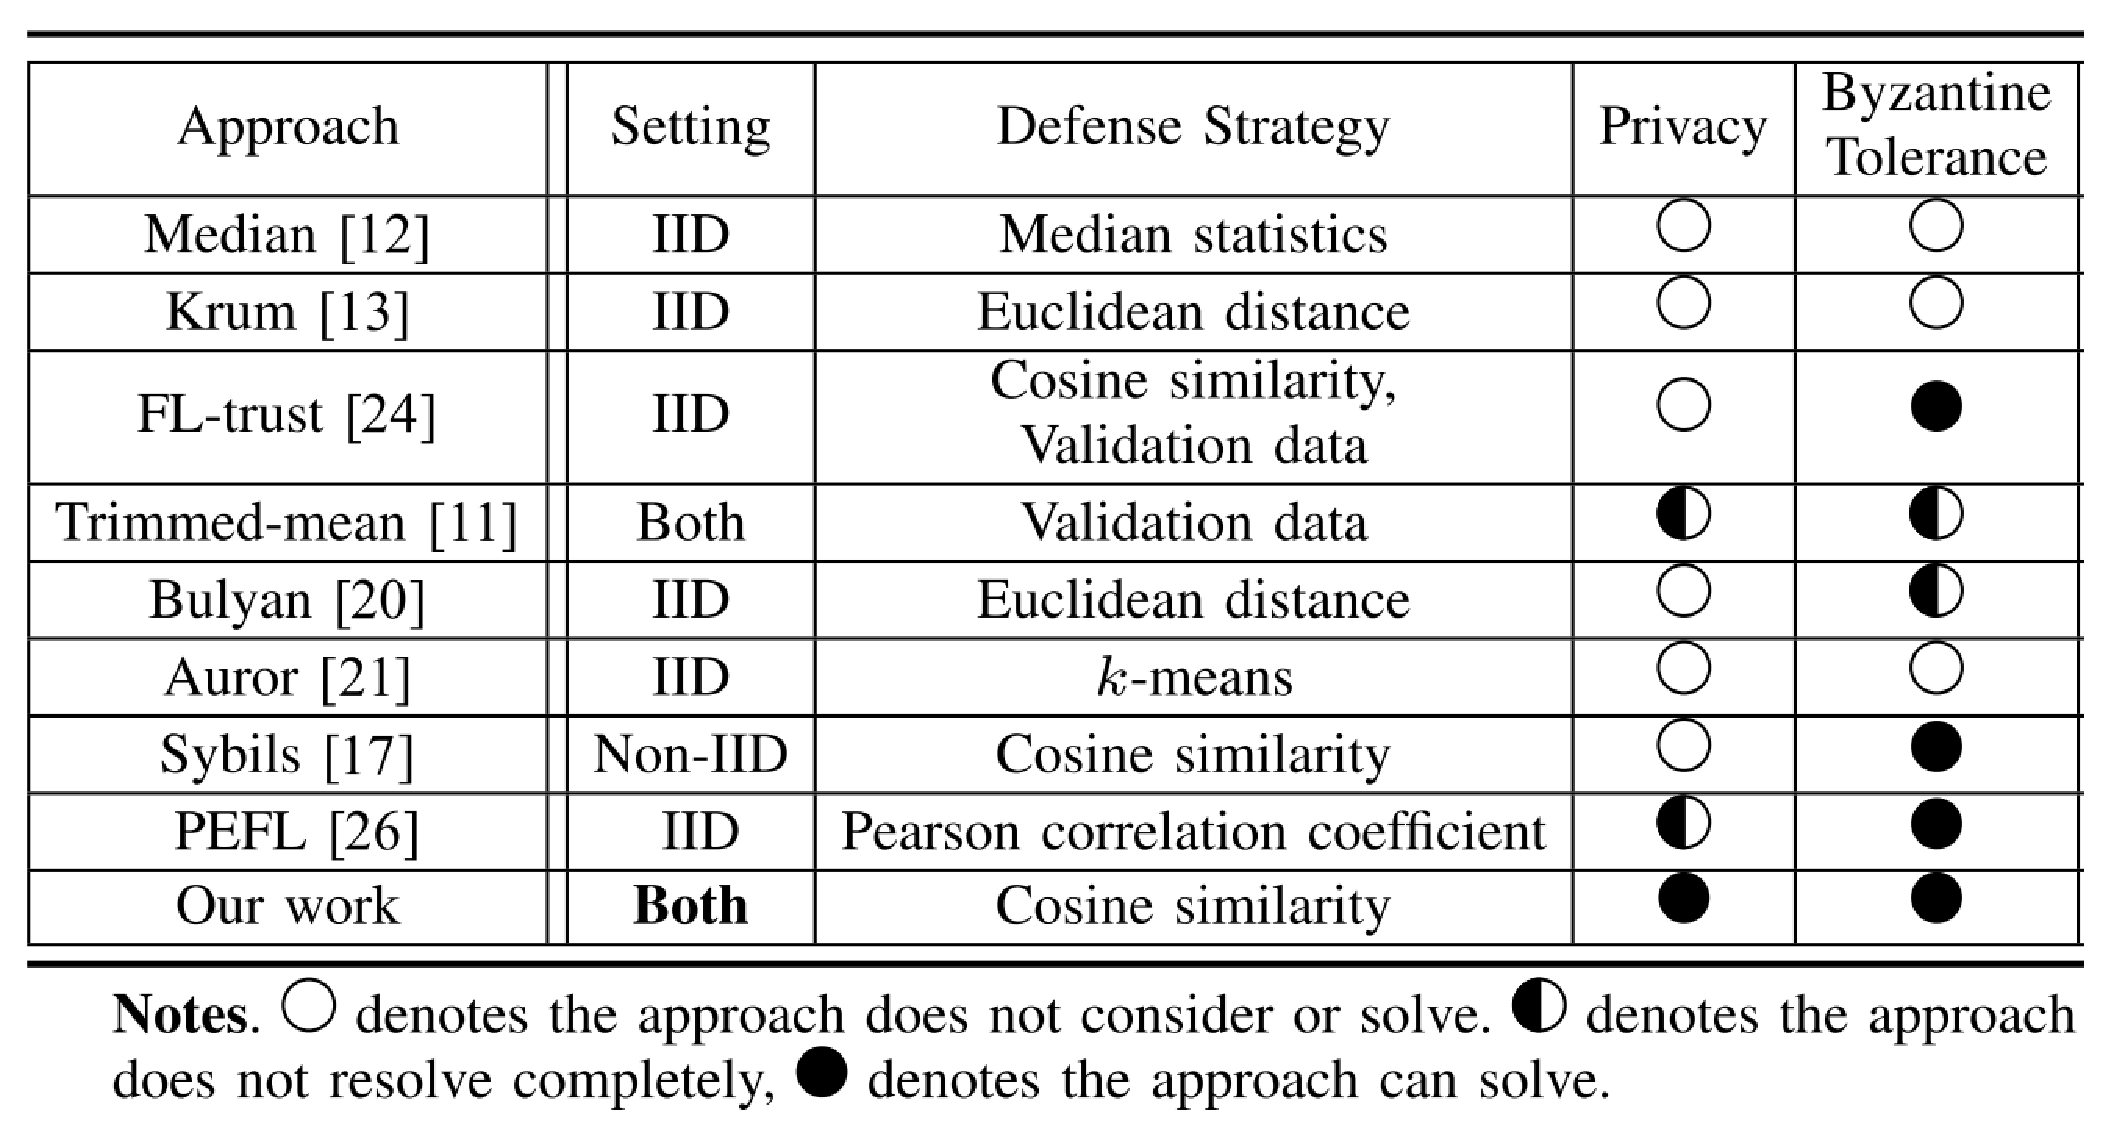
\includegraphics[width=0.8\linewidth]{resources/state-of-the-art-comarison.pdf}
  \caption{A comparative summary of existing defense strategies}
  \label{fig:comparison-with-state-of-the-art-schemes}
  %\vspace{-5mm}
\end{figure}


\vspace{-5mm}
\subsection{Contributions}

To address these challenges, we introduce ShieldFL, a privacy-preserving defense strategy against model poisoning attacks in \ac{ppfl}.
% ShieldFL leverages a two-trapdoor \ac{he} mechanism to safeguard against key disclosure and data leakage, ensuring robust data privacy.
Our approach begins with a privacy-preserving defense strategy utilizing cosine similarity to counter encrypted model poisoning in \ac{ppfl}.
% Additionally, we devise a Byzantine-tolerance aggregation mechanism tailored for heterogeneous data scenarios, enhancing the system's robustness.
The key contributions of ShieldFL include:
\begin{enumerate*}
    \item Introduction of a privacy-preserving defense strategy based on two-trapdoor \ac{he}, offering resilience against encrypted model poisoning.
    \item Design of a Byzantine-tolerance aggregation mechanism within ShieldFL to enhance robustness. This mechanism caters to heterogeneous data scenarios, accommodating both \ac{iid} and non-\ac{iid} data, with the goal of mitigating the impact of malicious users, comprising less than $50\%$ of the total.
    \item Evaluation of ShieldFL using three real-world datasets, assessing its performance against two representative model poisoning attacks: targeted and untargeted attacks. 
\end{enumerate*}